\section{Calibration}
Assuming the density is independent of $x$, i.e. $\sigma$ does not change along the swath width, equation \eqref{eq:integralDeDensidadEsflujoSobreRapidez} can be easily solved to obtain

\begin{equation}
  \sigma = \frac{\dot{m}}{s\cdot w}.
  \label{eq:densidadEsFlujoSobreProductoRapidezPorAncho}
\end{equation}

In order to write equation \eqref{eq:densidadEsFlujoSobreProductoRapidezPorAncho} as a function of the aperture diameter of the bait bucket, we express the mass flow rate of bait as a function of the aperture diameter, $\dot{m}(d)$. To do this, the bait in the bucket was weighed and the time required to empty the bucket was measured and repeated using several aperture diameters. Figure \ref{fig:flujoDeApertura} shows the results from the calibration as well as the fitted model.

\begin{figure}
  % Generada por plotFlow.m
  \centering
  \begin{subfigure}[b]{0.45\textwidth}
    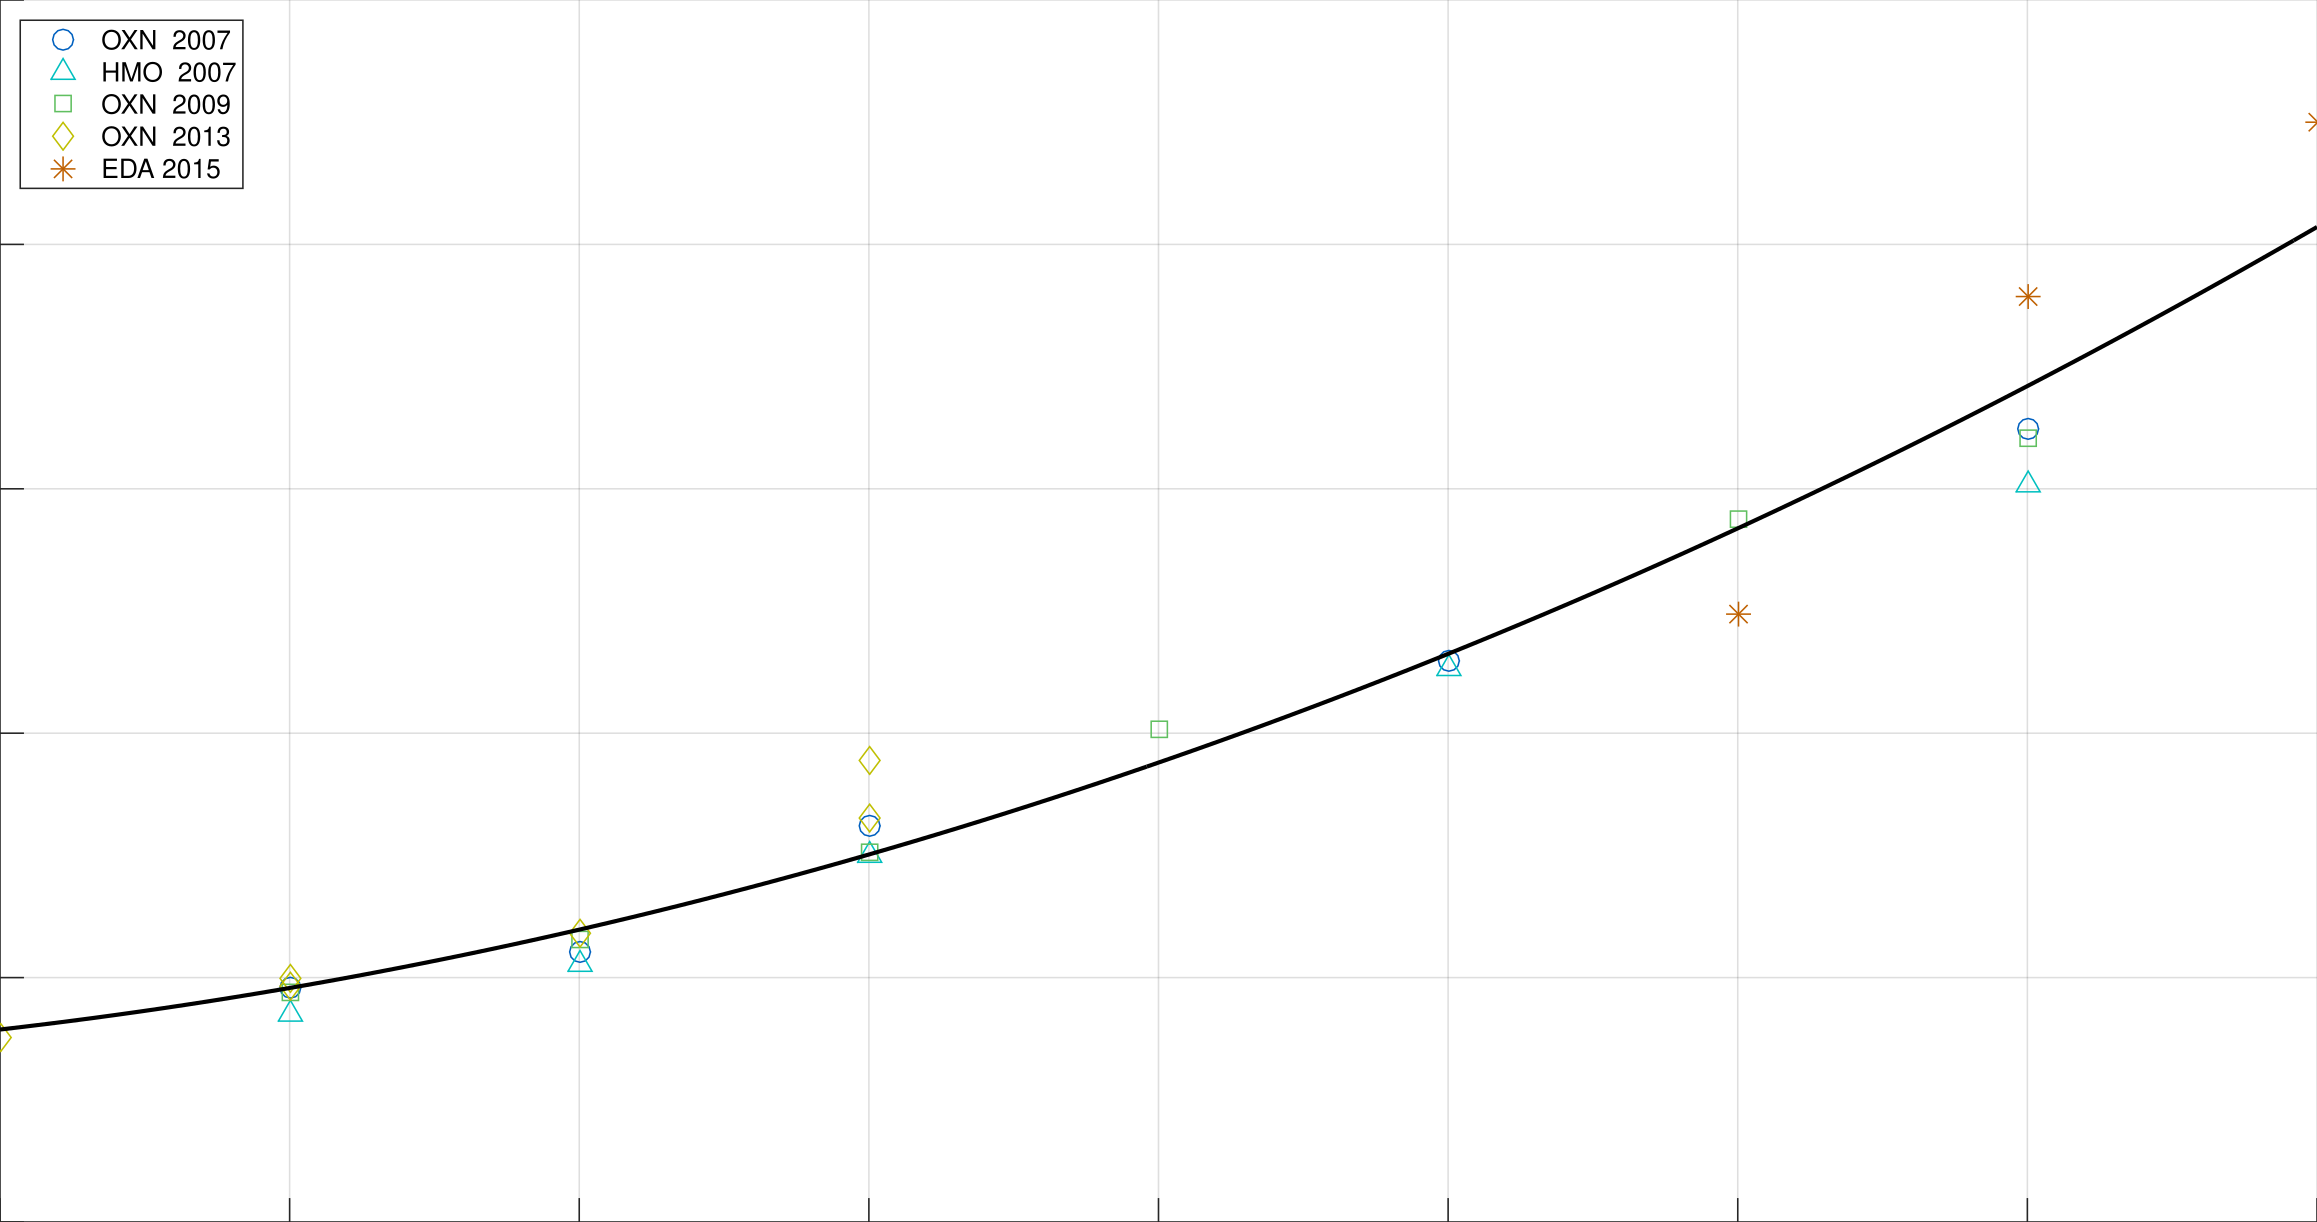
\includegraphics[width=\textwidth]{../resultados/png/flujo-de-apertura.png}
    \caption{$\dot{m}(d)$}
    \label{fig:flujoDeApertura}
  \end{subfigure}
  \begin{subfigure}[b]{0.45\textwidth}
    % Aquí­ va la figura generada a partir `images\density.svg`.
    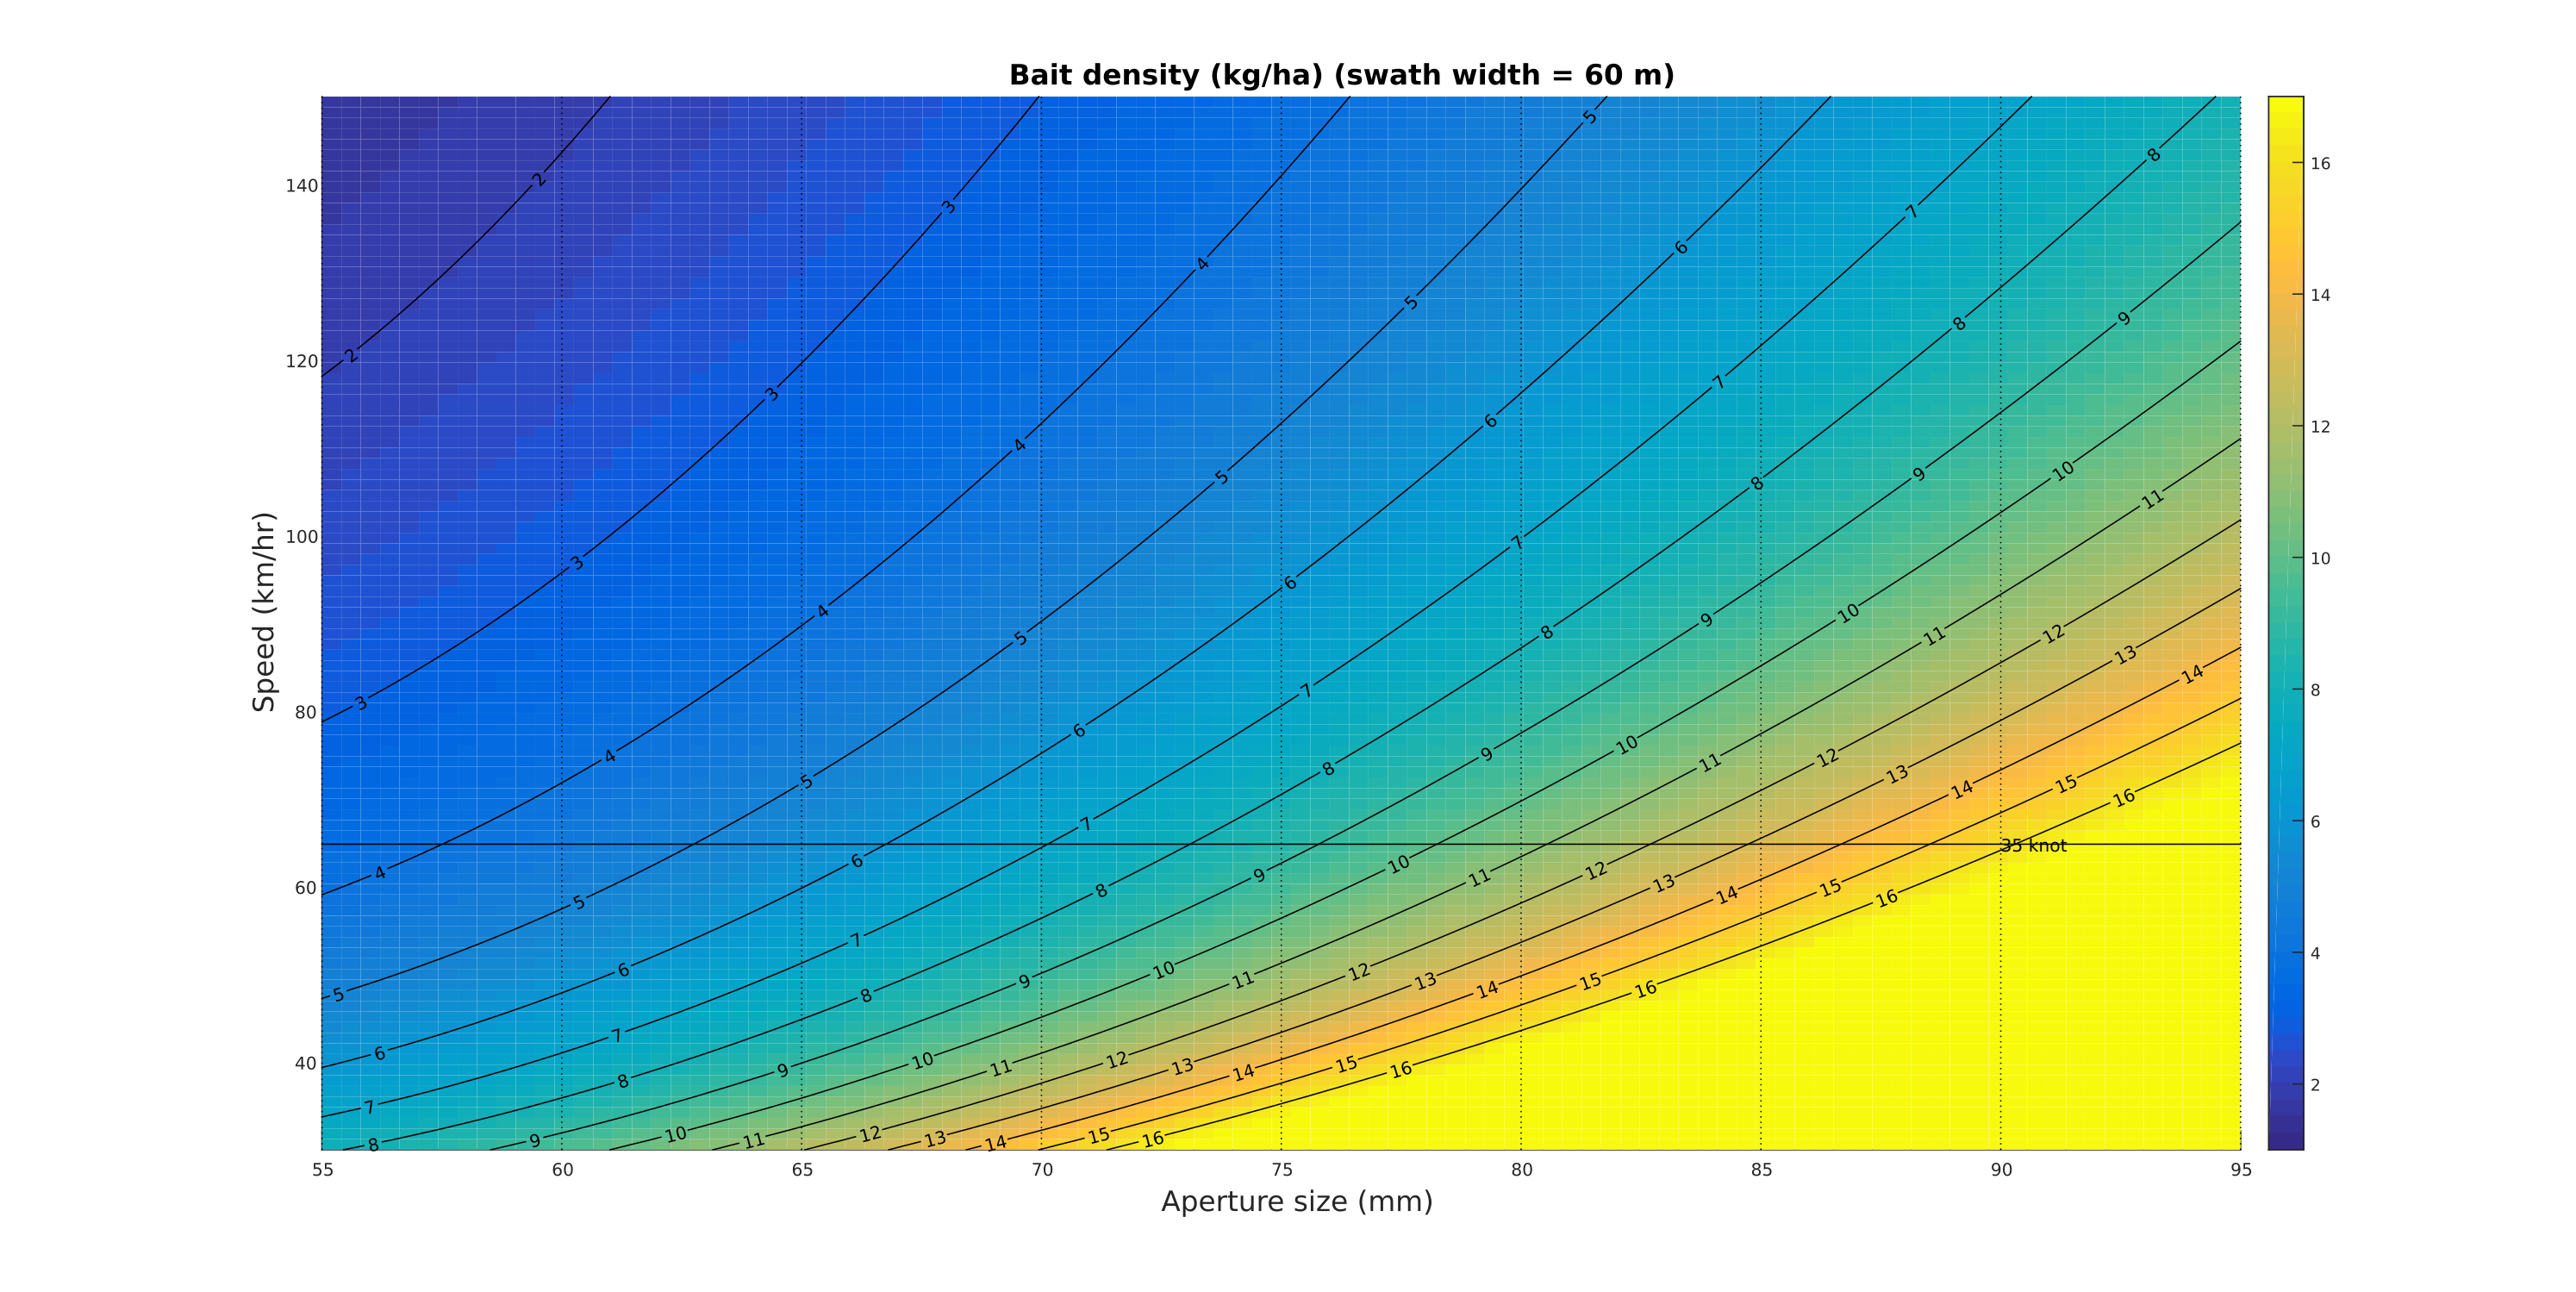
\includegraphics[width=\textwidth]{../resultados/png/densidad-de-apertura-y-rapidez.png}
    \caption{$\sigma(d,s)= \frac{\dot{m}(d)}{s\cdot w}$}
    \label{fig:densidadDeAperturaYRapidez}
  \end{subfigure}
  \caption{ \ref{fig:flujoDeApertura}
  Flow rate $\dot{m}$ (kg/s) as a function of aperture diameter, $d$
  (mm); each symbol represents a calibration event and the black curve is the
  quadratic model fitted to the data. \ref{fig:densidadDeAperturaYRapidez}
  Surface bait density $\sigma$ (kg/ha) as a function of aperture diameter $d$
  (mm), and speed $s$ (km/hr). The horizontal axis shows the aperture diameter of
  the bait bucket and the vertical axis shows the helicopter's speed. The
  resulting bait density on the ground is shown in the second vertical color axis.}
\end{figure}

The resulting three-dimensional model, $$\sigma(d,s)= \frac{\dot{m}(d)}{s\cdot w},$$ is shown in Figure \ref{fig:densidadDeAperturaYRapidez}. During the planning stage of an eradication campaign, this model can be used to determine the diameter of the bait bucket needed to achieve the desired bait density on the ground, ensuring efficient bait coverage, while maximizing resources, time and manpower.
